\chapter{Diagrama de actividades}

\begin{figure}[h!]
	\centering
	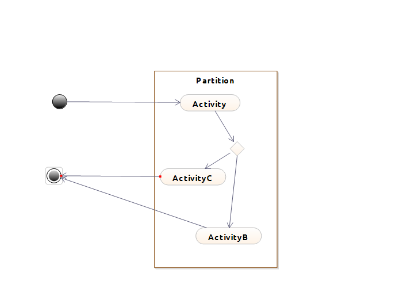
\includegraphics[scale=0.5]{diseno/actividades/img/actividades}
	\caption{Diagrama de Nodos}
\end{figure}

Esta herramienta es muy útil para entender cómo será el funcionamiento que va a tener el proyecto en ejecución, esto debido a que permite modelar el flujo que tendrán los diferentes procesos que se van a realizar dentro del mismo.
Este tipo de diagramas está fuertemente ligado con el diagrama de estados, debido a que en este diagrama, al igual que en el de estados contaremos con un estado inicial y uno final que indicarán dónde comienza y dónde termina el workflow

\section{Workflow}
Cuando se habla del workflow, es precisamente el modelamiento del flujo de trabajo y en esta parte aparecen dos elementos sumamente importantes: las actividades y las particiones.
Por un lado las particiones son las que indican los elementos o los participantes con los que se contará para el desarrollo de las actividades, mientras que estas últimas representan los procesos que se realizarán dentro del workflow.
Una de las principales características que tiene este diagrama es que tiene en cuenta las decisiones que se pueden presentar a lo largo del programa, y a partir de estas define el flujo que él mismo tomará para funcionar.

\section{Cine+}
Para el aplicativo que se está realizando de Cine+ se detectaron los siguientes diagramas de estado, cada uno correspondiente a cada uno de las partes del aplicativo: administrativo y cliente.
\subsection*{Aplicativo Cliente}
\begin{figure}[h!]
	\centering
	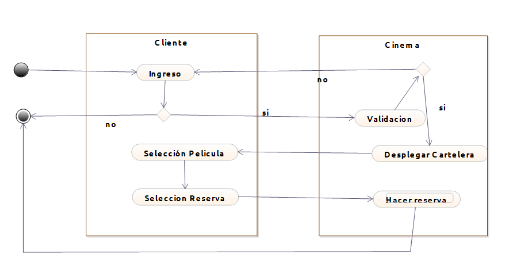
\includegraphics[scale=0.5]{diseno/actividades/img/actividadesCliente}
	\caption{Diagrama de Nodos}
\end{figure}

\subsection*{Aplicativo Administrativo}
\begin{figure}[h!]
	\centering
	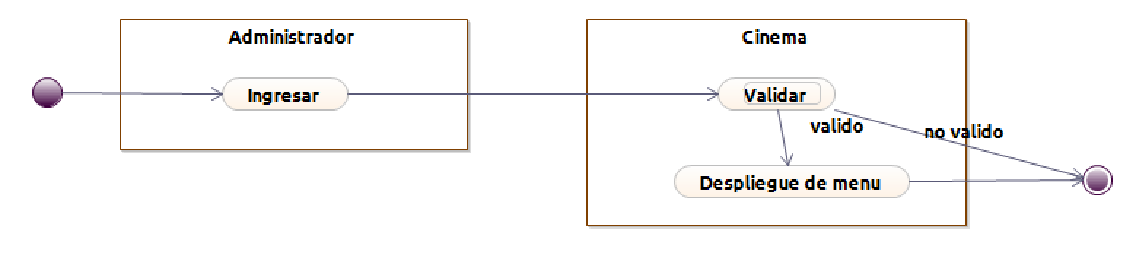
\includegraphics[scale=0.5]{diseno/actividades/img/inicio}
	\caption{Diagrama de actividades Aplicativo Administrativo}
\end{figure}


\begin{figure}[h!]
	\centering
	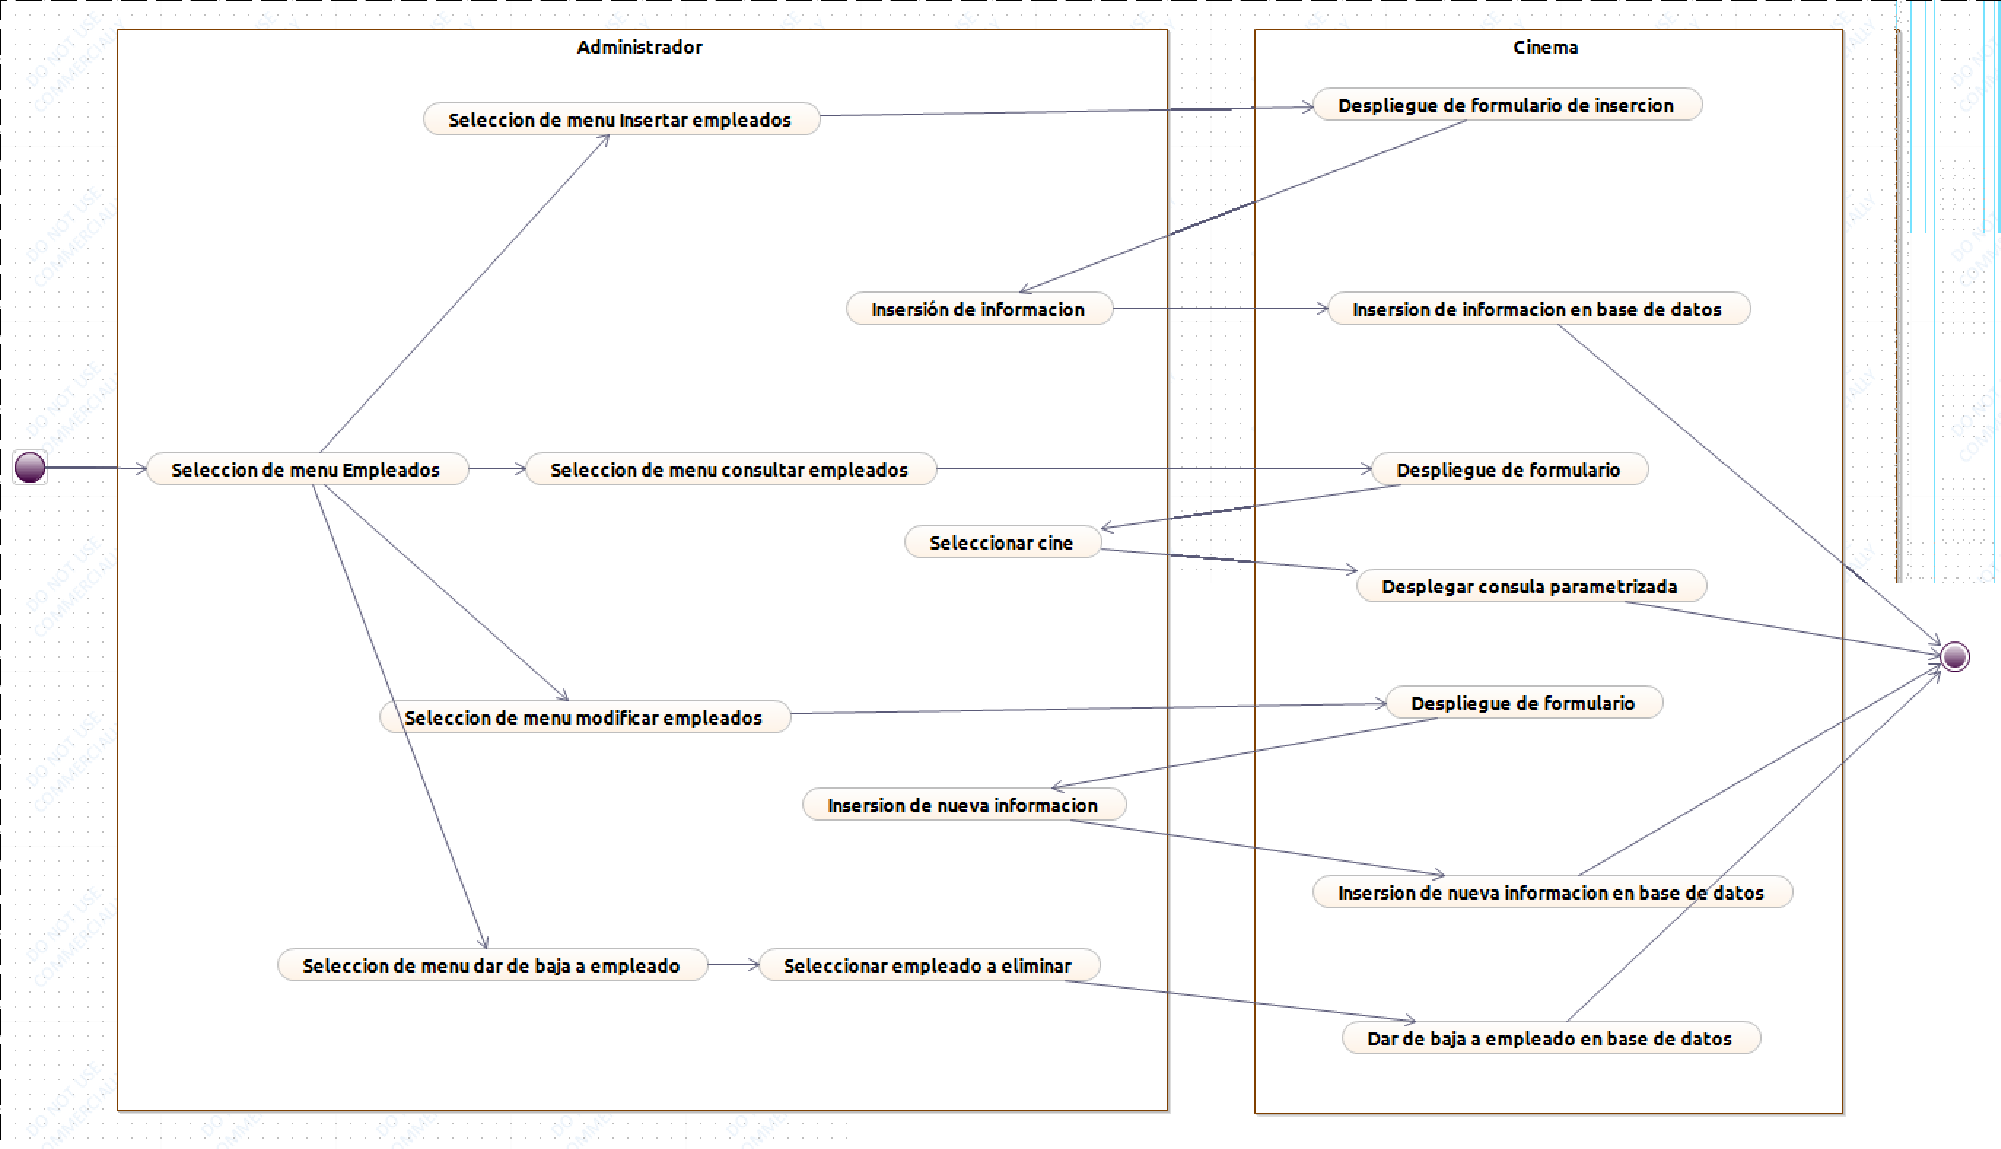
\includegraphics[scale=0.4]{diseno/actividades/img/empleados}
	\caption{Diagrama de actividades Módulo Empleados}
\end{figure}

\begin{figure}[h!]
	\centering
	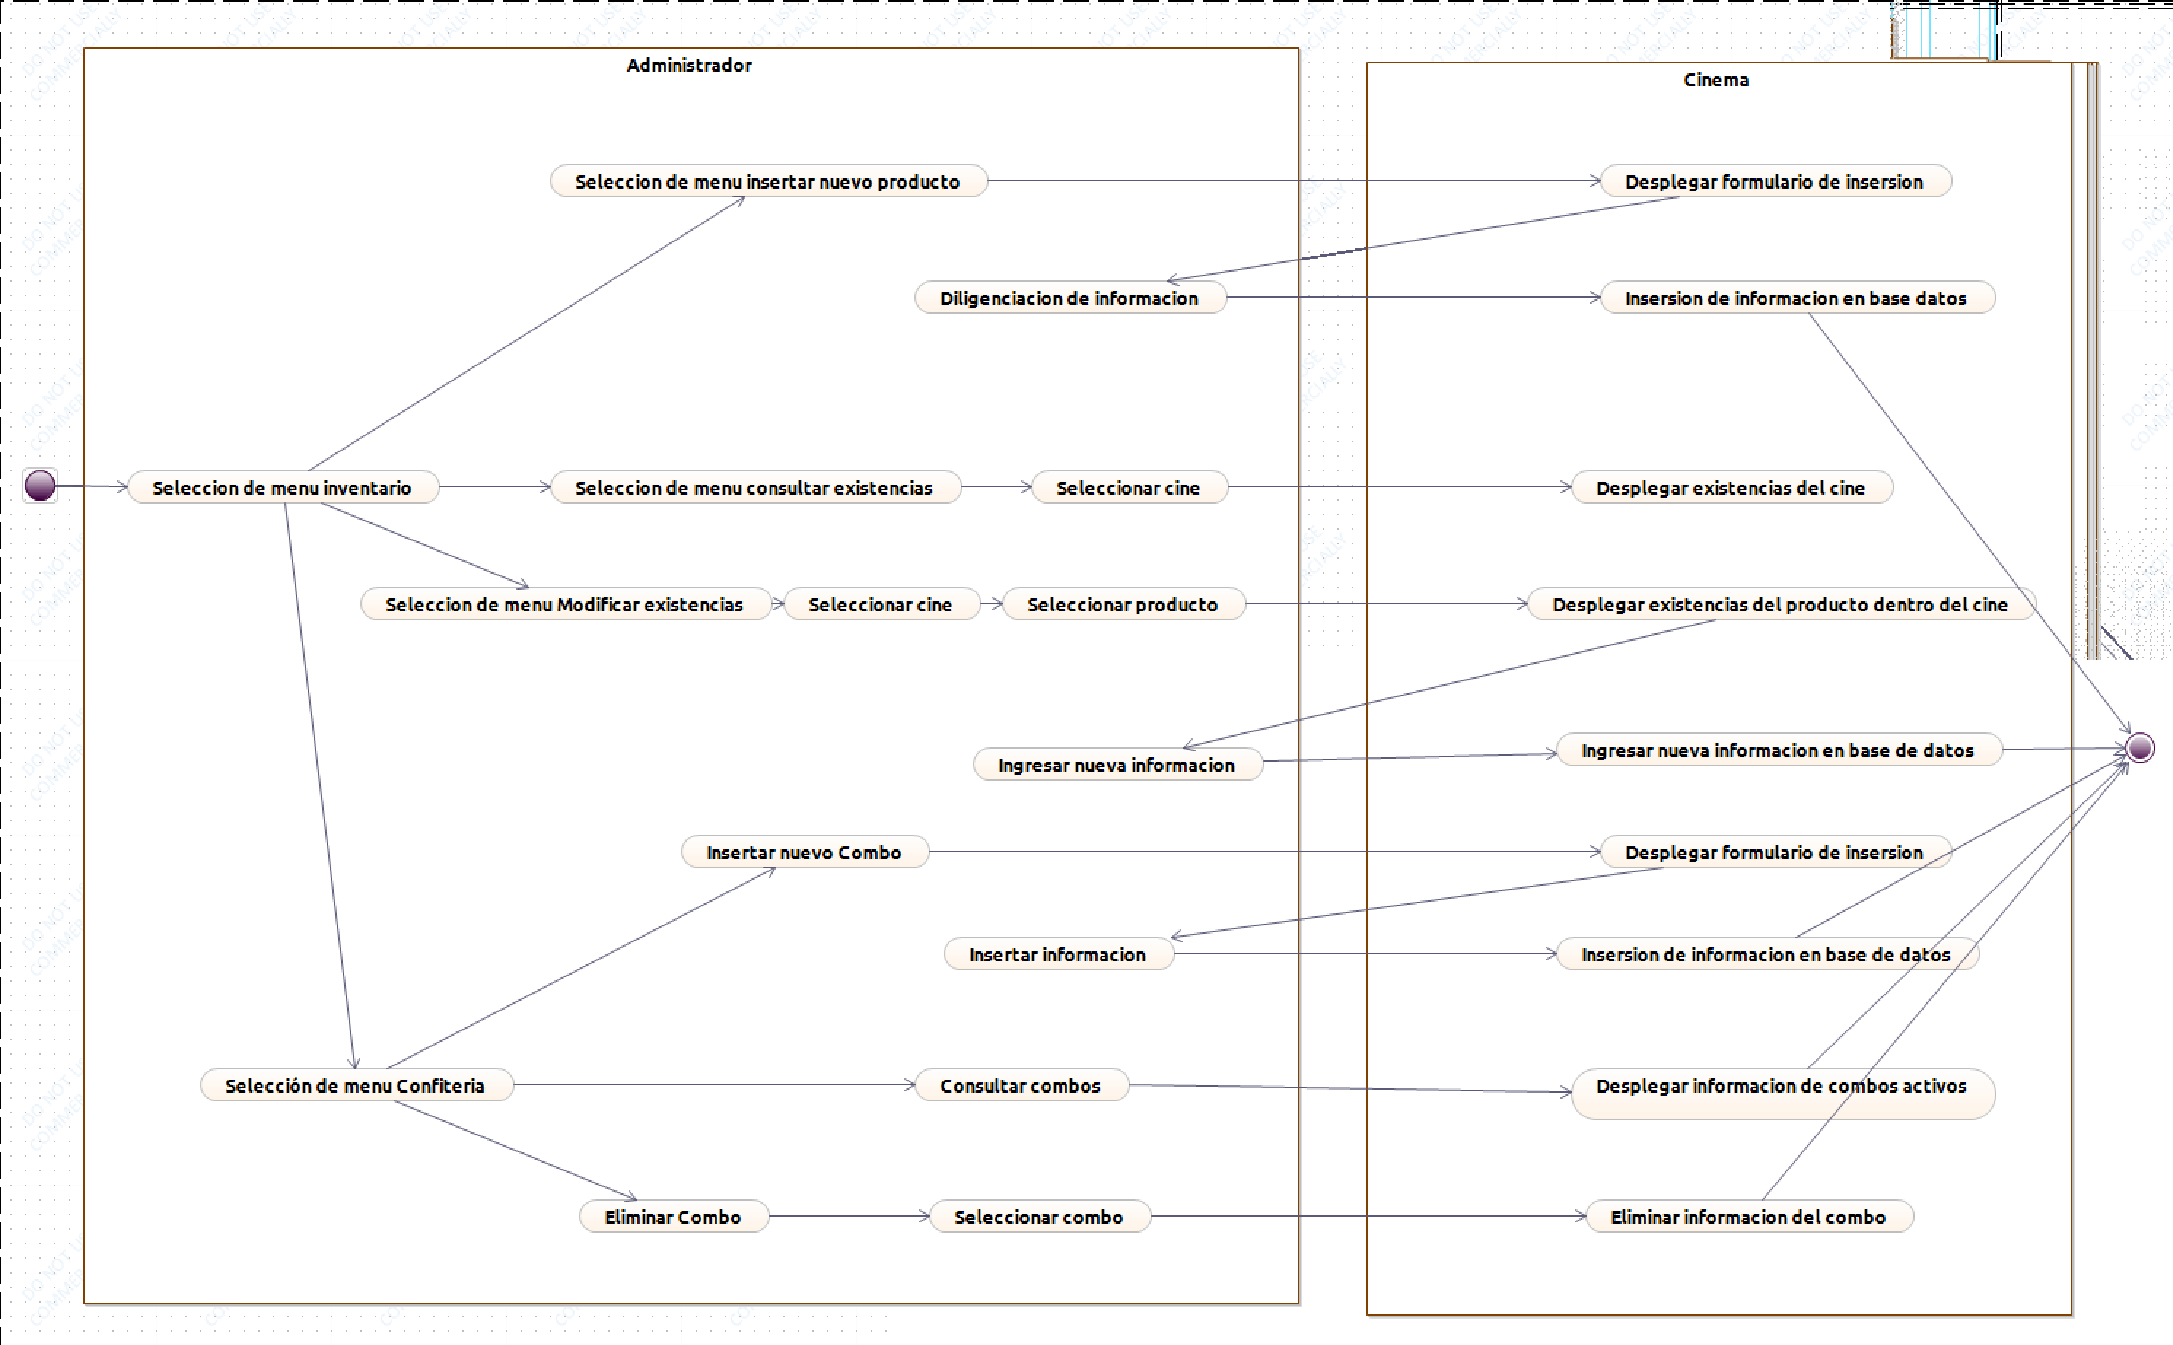
\includegraphics[scale=0.4]{diseno/actividades/img/inventario}
	\caption{Diagrama de actividades Módulo Inventario}
\end{figure}

\begin{figure}[h!]
	\centering
	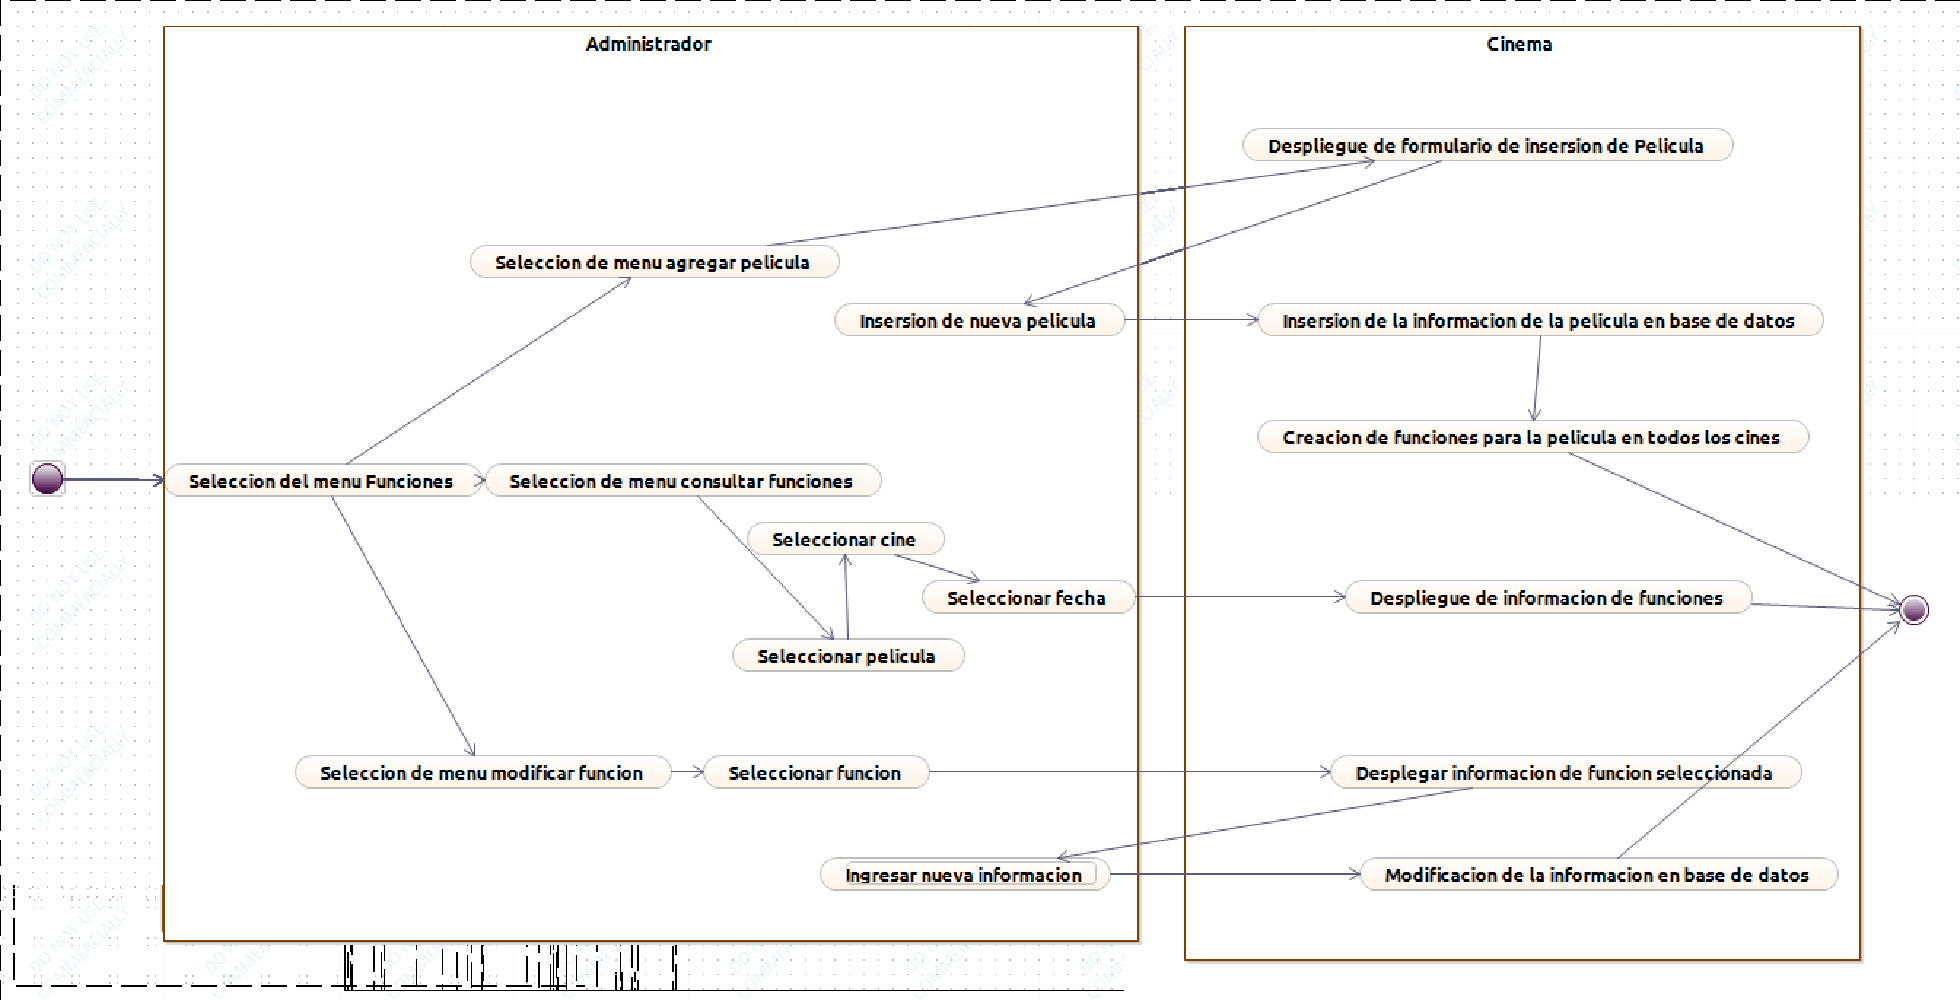
\includegraphics[scale=0.4]{diseno/actividades/img/funciones}
	\caption{Diagrama de actividades Módulo Funciones}
\end{figure}